% Created by tikzDevice version 0.10.1 on 2017-10-30 17:28:50
% !TEX encoding = UTF-8 Unicode
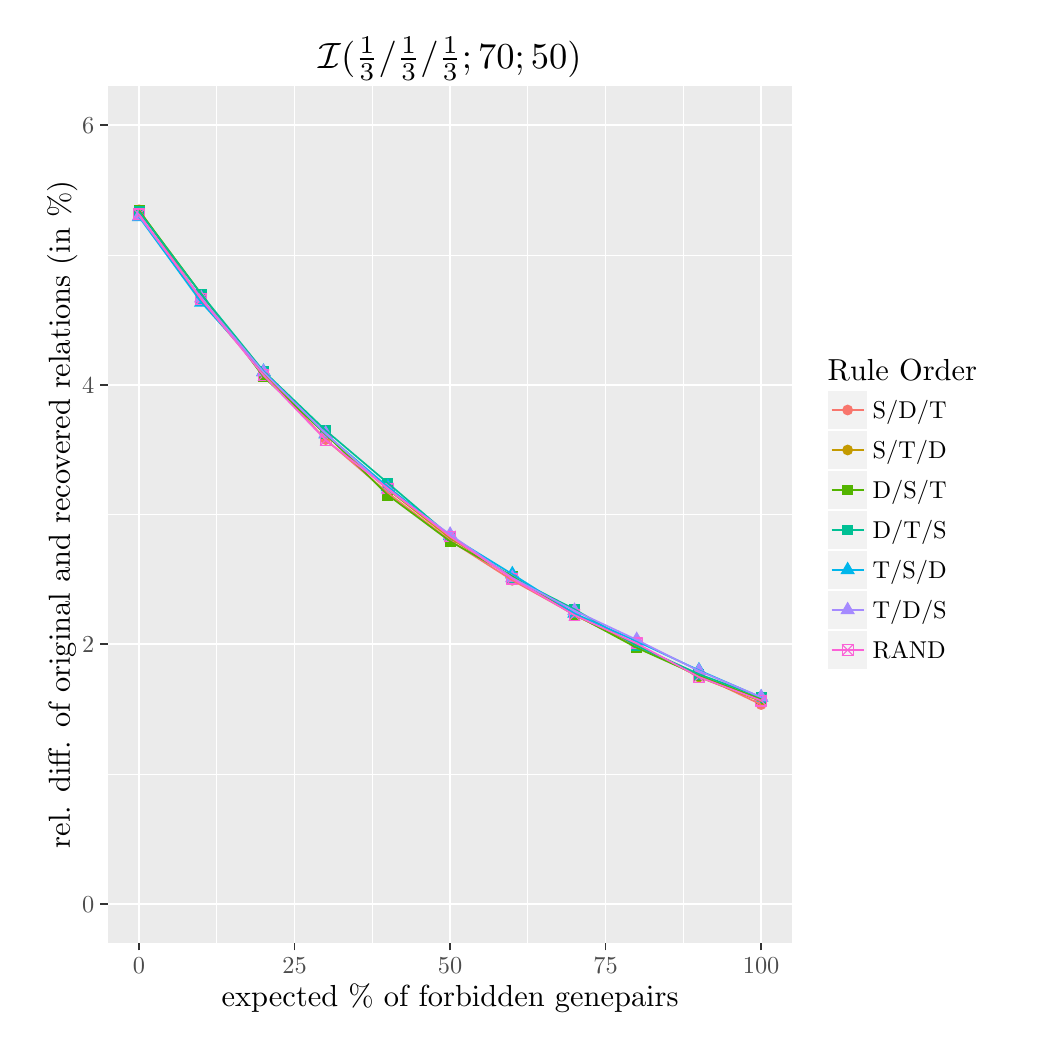
\begin{tikzpicture}[x=1pt,y=1pt]
\definecolor{fillColor}{RGB}{255,255,255}
\path[use as bounding box,fill=fillColor,fill opacity=0.00] (0,0) rectangle (361.35,361.35);
\begin{scope}
\path[clip] (  0.00,  0.00) rectangle (361.35,361.35);
\definecolor{drawColor}{RGB}{255,255,255}
\definecolor{fillColor}{RGB}{255,255,255}

\path[draw=drawColor,line width= 0.6pt,line join=round,line cap=round,fill=fillColor] (  0.00,  0.00) rectangle (361.35,361.35);
\end{scope}
\begin{scope}
\path[clip] ( 29.02, 30.69) rectangle (276.26,340.16);
\definecolor{fillColor}{gray}{0.92}

\path[fill=fillColor] ( 29.02, 30.69) rectangle (276.26,340.16);
\definecolor{drawColor}{RGB}{255,255,255}

\path[draw=drawColor,line width= 0.3pt,line join=round] ( 29.02, 91.64) --
	(276.26, 91.64);

\path[draw=drawColor,line width= 0.3pt,line join=round] ( 29.02,185.42) --
	(276.26,185.42);

\path[draw=drawColor,line width= 0.3pt,line join=round] ( 29.02,279.20) --
	(276.26,279.20);

\path[draw=drawColor,line width= 0.3pt,line join=round] ( 68.36, 30.69) --
	( 68.36,340.16);

\path[draw=drawColor,line width= 0.3pt,line join=round] (124.55, 30.69) --
	(124.55,340.16);

\path[draw=drawColor,line width= 0.3pt,line join=round] (180.74, 30.69) --
	(180.74,340.16);

\path[draw=drawColor,line width= 0.3pt,line join=round] (236.93, 30.69) --
	(236.93,340.16);

\path[draw=drawColor,line width= 0.6pt,line join=round] ( 29.02, 44.75) --
	(276.26, 44.75);

\path[draw=drawColor,line width= 0.6pt,line join=round] ( 29.02,138.53) --
	(276.26,138.53);

\path[draw=drawColor,line width= 0.6pt,line join=round] ( 29.02,232.31) --
	(276.26,232.31);

\path[draw=drawColor,line width= 0.6pt,line join=round] ( 29.02,326.09) --
	(276.26,326.09);

\path[draw=drawColor,line width= 0.6pt,line join=round] ( 40.26, 30.69) --
	( 40.26,340.16);

\path[draw=drawColor,line width= 0.6pt,line join=round] ( 96.45, 30.69) --
	( 96.45,340.16);

\path[draw=drawColor,line width= 0.6pt,line join=round] (152.64, 30.69) --
	(152.64,340.16);

\path[draw=drawColor,line width= 0.6pt,line join=round] (208.83, 30.69) --
	(208.83,340.16);

\path[draw=drawColor,line width= 0.6pt,line join=round] (265.03, 30.69) --
	(265.03,340.16);
\definecolor{fillColor}{RGB}{248,118,109}

\path[fill=fillColor] ( 40.26,295.54) circle (  1.96);

\path[fill=fillColor] ( 62.74,263.14) circle (  1.96);

\path[fill=fillColor] ( 85.22,236.63) circle (  1.96);

\path[fill=fillColor] (107.69,212.50) circle (  1.96);

\path[fill=fillColor] (130.17,193.23) circle (  1.96);

\path[fill=fillColor] (152.64,176.03) circle (  1.96);

\path[fill=fillColor] (175.12,161.65) circle (  1.96);

\path[fill=fillColor] (197.60,149.22) circle (  1.96);

\path[fill=fillColor] (220.07,137.81) circle (  1.96);

\path[fill=fillColor] (242.55,127.52) circle (  1.96);

\path[fill=fillColor] (265.03,116.75) circle (  1.96);
\definecolor{fillColor}{RGB}{196,154,0}

\path[fill=fillColor] ( 40.26,293.55) circle (  1.96);

\path[fill=fillColor] ( 62.74,262.65) circle (  1.96);

\path[fill=fillColor] ( 85.22,236.37) circle (  1.96);

\path[fill=fillColor] (107.69,214.20) circle (  1.96);

\path[fill=fillColor] (130.17,194.46) circle (  1.96);

\path[fill=fillColor] (152.64,176.89) circle (  1.96);

\path[fill=fillColor] (175.12,162.92) circle (  1.96);

\path[fill=fillColor] (197.60,149.00) circle (  1.96);

\path[fill=fillColor] (220.07,138.54) circle (  1.96);

\path[fill=fillColor] (242.55,126.72) circle (  1.96);

\path[fill=fillColor] (265.03,117.93) circle (  1.96);
\definecolor{fillColor}{RGB}{83,180,0}

\path[fill=fillColor] ( 38.30,293.29) --
	( 42.23,293.29) --
	( 42.23,297.22) --
	( 38.30,297.22) --
	cycle;

\path[fill=fillColor] ( 60.78,263.15) --
	( 64.70,263.15) --
	( 64.70,267.07) --
	( 60.78,267.07) --
	cycle;

\path[fill=fillColor] ( 83.25,233.21) --
	( 87.18,233.21) --
	( 87.18,237.13) --
	( 83.25,237.13) --
	cycle;

\path[fill=fillColor] (105.73,212.55) --
	(109.65,212.55) --
	(109.65,216.47) --
	(105.73,216.47) --
	cycle;

\path[fill=fillColor] (128.21,190.47) --
	(132.13,190.47) --
	(132.13,194.39) --
	(128.21,194.39) --
	cycle;

\path[fill=fillColor] (150.68,173.78) --
	(154.61,173.78) --
	(154.61,177.70) --
	(150.68,177.70) --
	cycle;

\path[fill=fillColor] (173.16,161.15) --
	(177.08,161.15) --
	(177.08,165.08) --
	(173.16,165.08) --
	cycle;

\path[fill=fillColor] (195.63,147.41) --
	(199.56,147.41) --
	(199.56,151.33) --
	(195.63,151.33) --
	cycle;

\path[fill=fillColor] (218.11,135.31) --
	(222.04,135.31) --
	(222.04,139.24) --
	(218.11,139.24) --
	cycle;

\path[fill=fillColor] (240.59,125.22) --
	(244.51,125.22) --
	(244.51,129.15) --
	(240.59,129.15) --
	cycle;

\path[fill=fillColor] (263.06,116.81) --
	(266.99,116.81) --
	(266.99,120.73) --
	(263.06,120.73) --
	cycle;
\definecolor{fillColor}{RGB}{0,192,148}

\path[fill=fillColor] ( 38.30,292.88) --
	( 42.23,292.88) --
	( 42.23,296.80) --
	( 38.30,296.80) --
	cycle;

\path[fill=fillColor] ( 60.78,263.04) --
	( 64.70,263.04) --
	( 64.70,266.96) --
	( 60.78,266.96) --
	cycle;

\path[fill=fillColor] ( 83.25,235.31) --
	( 87.18,235.31) --
	( 87.18,239.23) --
	( 83.25,239.23) --
	cycle;

\path[fill=fillColor] (105.73,213.84) --
	(109.65,213.84) --
	(109.65,217.77) --
	(105.73,217.77) --
	cycle;

\path[fill=fillColor] (128.21,194.81) --
	(132.13,194.81) --
	(132.13,198.73) --
	(128.21,198.73) --
	cycle;

\path[fill=fillColor] (150.68,175.65) --
	(154.61,175.65) --
	(154.61,179.58) --
	(150.68,179.58) --
	cycle;

\path[fill=fillColor] (173.16,160.72) --
	(177.08,160.72) --
	(177.08,164.64) --
	(173.16,164.64) --
	cycle;

\path[fill=fillColor] (195.63,149.24) --
	(199.56,149.24) --
	(199.56,153.16) --
	(195.63,153.16) --
	cycle;

\path[fill=fillColor] (218.11,136.02) --
	(222.04,136.02) --
	(222.04,139.94) --
	(218.11,139.94) --
	cycle;

\path[fill=fillColor] (240.59,125.80) --
	(244.51,125.80) --
	(244.51,129.72) --
	(240.59,129.72) --
	cycle;

\path[fill=fillColor] (263.06,117.41) --
	(266.99,117.41) --
	(266.99,121.33) --
	(263.06,121.33) --
	cycle;
\definecolor{fillColor}{RGB}{0,182,235}

\path[fill=fillColor] ( 40.26,295.98) --
	( 42.91,291.40) --
	( 37.62,291.40) --
	cycle;

\path[fill=fillColor] ( 62.74,265.14) --
	( 65.38,260.56) --
	( 60.10,260.56) --
	cycle;

\path[fill=fillColor] ( 85.22,240.13) --
	( 87.86,235.55) --
	( 82.57,235.55) --
	cycle;

\path[fill=fillColor] (107.69,217.54) --
	(110.33,212.96) --
	(105.05,212.96) --
	cycle;

\path[fill=fillColor] (130.17,198.46) --
	(132.81,193.88) --
	(127.53,193.88) --
	cycle;

\path[fill=fillColor] (152.64,180.73) --
	(155.29,176.16) --
	(150.00,176.16) --
	cycle;

\path[fill=fillColor] (175.12,166.94) --
	(177.76,162.36) --
	(172.48,162.36) --
	cycle;

\path[fill=fillColor] (197.60,152.72) --
	(200.24,148.15) --
	(194.95,148.15) --
	cycle;

\path[fill=fillColor] (220.07,142.68) --
	(222.72,138.10) --
	(217.43,138.10) --
	cycle;

\path[fill=fillColor] (242.55,132.20) --
	(245.19,127.63) --
	(239.91,127.63) --
	cycle;

\path[fill=fillColor] (265.03,122.41) --
	(267.67,117.83) --
	(262.38,117.83) --
	cycle;
\definecolor{fillColor}{RGB}{165,138,255}

\path[fill=fillColor] ( 40.26,296.29) --
	( 42.91,291.71) --
	( 37.62,291.71) --
	cycle;

\path[fill=fillColor] ( 62.74,266.70) --
	( 65.38,262.12) --
	( 60.10,262.12) --
	cycle;

\path[fill=fillColor] ( 85.22,239.93) --
	( 87.86,235.35) --
	( 82.57,235.35) --
	cycle;

\path[fill=fillColor] (107.69,217.76) --
	(110.33,213.18) --
	(105.05,213.18) --
	cycle;

\path[fill=fillColor] (130.17,197.58) --
	(132.81,193.00) --
	(127.53,193.00) --
	cycle;

\path[fill=fillColor] (152.64,181.26) --
	(155.29,176.68) --
	(150.00,176.68) --
	cycle;

\path[fill=fillColor] (175.12,165.58) --
	(177.76,161.00) --
	(172.48,161.00) --
	cycle;

\path[fill=fillColor] (197.60,153.72) --
	(200.24,149.15) --
	(194.95,149.15) --
	cycle;

\path[fill=fillColor] (220.07,143.21) --
	(222.72,138.63) --
	(217.43,138.63) --
	cycle;

\path[fill=fillColor] (242.55,131.95) --
	(245.19,127.37) --
	(239.91,127.37) --
	cycle;

\path[fill=fillColor] (265.03,122.49) --
	(267.67,117.91) --
	(262.38,117.91) --
	cycle;
\definecolor{drawColor}{RGB}{251,97,215}

\path[draw=drawColor,line width= 0.4pt,line join=round,line cap=round] ( 38.30,291.89) rectangle ( 42.23,295.81);

\path[draw=drawColor,line width= 0.4pt,line join=round,line cap=round] ( 38.30,291.89) -- ( 42.23,295.81);

\path[draw=drawColor,line width= 0.4pt,line join=round,line cap=round] ( 38.30,295.81) -- ( 42.23,291.89);

\path[draw=drawColor,line width= 0.4pt,line join=round,line cap=round] ( 60.78,261.27) rectangle ( 64.70,265.20);

\path[draw=drawColor,line width= 0.4pt,line join=round,line cap=round] ( 60.78,261.27) -- ( 64.70,265.20);

\path[draw=drawColor,line width= 0.4pt,line join=round,line cap=round] ( 60.78,265.20) -- ( 64.70,261.27);

\path[draw=drawColor,line width= 0.4pt,line join=round,line cap=round] ( 83.25,233.75) rectangle ( 87.18,237.67);

\path[draw=drawColor,line width= 0.4pt,line join=round,line cap=round] ( 83.25,233.75) -- ( 87.18,237.67);

\path[draw=drawColor,line width= 0.4pt,line join=round,line cap=round] ( 83.25,237.67) -- ( 87.18,233.75);

\path[draw=drawColor,line width= 0.4pt,line join=round,line cap=round] (105.73,210.38) rectangle (109.65,214.31);

\path[draw=drawColor,line width= 0.4pt,line join=round,line cap=round] (105.73,210.38) -- (109.65,214.31);

\path[draw=drawColor,line width= 0.4pt,line join=round,line cap=round] (105.73,214.31) -- (109.65,210.38);

\path[draw=drawColor,line width= 0.4pt,line join=round,line cap=round] (128.21,192.86) rectangle (132.13,196.78);

\path[draw=drawColor,line width= 0.4pt,line join=round,line cap=round] (128.21,192.86) -- (132.13,196.78);

\path[draw=drawColor,line width= 0.4pt,line join=round,line cap=round] (128.21,196.78) -- (132.13,192.86);

\path[draw=drawColor,line width= 0.4pt,line join=round,line cap=round] (150.68,175.52) rectangle (154.61,179.45);

\path[draw=drawColor,line width= 0.4pt,line join=round,line cap=round] (150.68,175.52) -- (154.61,179.45);

\path[draw=drawColor,line width= 0.4pt,line join=round,line cap=round] (150.68,179.45) -- (154.61,175.52);

\path[draw=drawColor,line width= 0.4pt,line join=round,line cap=round] (173.16,160.32) rectangle (177.08,164.25);

\path[draw=drawColor,line width= 0.4pt,line join=round,line cap=round] (173.16,160.32) -- (177.08,164.25);

\path[draw=drawColor,line width= 0.4pt,line join=round,line cap=round] (173.16,164.25) -- (177.08,160.32);

\path[draw=drawColor,line width= 0.4pt,line join=round,line cap=round] (195.63,147.10) rectangle (199.56,151.03);

\path[draw=drawColor,line width= 0.4pt,line join=round,line cap=round] (195.63,147.10) -- (199.56,151.03);

\path[draw=drawColor,line width= 0.4pt,line join=round,line cap=round] (195.63,151.03) -- (199.56,147.10);

\path[draw=drawColor,line width= 0.4pt,line join=round,line cap=round] (218.11,136.88) rectangle (222.04,140.80);

\path[draw=drawColor,line width= 0.4pt,line join=round,line cap=round] (218.11,136.88) -- (222.04,140.80);

\path[draw=drawColor,line width= 0.4pt,line join=round,line cap=round] (218.11,140.80) -- (222.04,136.88);

\path[draw=drawColor,line width= 0.4pt,line join=round,line cap=round] (240.59,124.78) rectangle (244.51,128.70);

\path[draw=drawColor,line width= 0.4pt,line join=round,line cap=round] (240.59,124.78) -- (244.51,128.70);

\path[draw=drawColor,line width= 0.4pt,line join=round,line cap=round] (240.59,128.70) -- (244.51,124.78);

\path[draw=drawColor,line width= 0.4pt,line join=round,line cap=round] (263.06,116.25) rectangle (266.99,120.17);

\path[draw=drawColor,line width= 0.4pt,line join=round,line cap=round] (263.06,116.25) -- (266.99,120.17);

\path[draw=drawColor,line width= 0.4pt,line join=round,line cap=round] (263.06,120.17) -- (266.99,116.25);
\definecolor{drawColor}{RGB}{248,118,109}

\path[draw=drawColor,line width= 0.6pt,line join=round] ( 40.26,295.54) --
	( 62.74,263.14) --
	( 85.22,236.63) --
	(107.69,212.50) --
	(130.17,193.23) --
	(152.64,176.03) --
	(175.12,161.65) --
	(197.60,149.22) --
	(220.07,137.81) --
	(242.55,127.52) --
	(265.03,116.75);
\definecolor{drawColor}{RGB}{196,154,0}

\path[draw=drawColor,line width= 0.6pt,line join=round] ( 40.26,293.55) --
	( 62.74,262.65) --
	( 85.22,236.37) --
	(107.69,214.20) --
	(130.17,194.46) --
	(152.64,176.89) --
	(175.12,162.92) --
	(197.60,149.00) --
	(220.07,138.54) --
	(242.55,126.72) --
	(265.03,117.93);
\definecolor{drawColor}{RGB}{83,180,0}

\path[draw=drawColor,line width= 0.6pt,line join=round] ( 40.26,295.26) --
	( 62.74,265.11) --
	( 85.22,235.17) --
	(107.69,214.51) --
	(130.17,192.43) --
	(152.64,175.74) --
	(175.12,163.11) --
	(197.60,149.37) --
	(220.07,137.27) --
	(242.55,127.18) --
	(265.03,118.77);
\definecolor{drawColor}{RGB}{0,192,148}

\path[draw=drawColor,line width= 0.6pt,line join=round] ( 40.26,294.84) --
	( 62.74,265.00) --
	( 85.22,237.27) --
	(107.69,215.80) --
	(130.17,196.77) --
	(152.64,177.61) --
	(175.12,162.68) --
	(197.60,151.20) --
	(220.07,137.98) --
	(242.55,127.76) --
	(265.03,119.37);
\definecolor{drawColor}{RGB}{0,182,235}

\path[draw=drawColor,line width= 0.6pt,line join=round] ( 40.26,292.93) --
	( 62.74,262.09) --
	( 85.22,237.07) --
	(107.69,214.49) --
	(130.17,195.41) --
	(152.64,177.68) --
	(175.12,163.89) --
	(197.60,149.67) --
	(220.07,139.62) --
	(242.55,129.15) --
	(265.03,119.36);
\definecolor{drawColor}{RGB}{165,138,255}

\path[draw=drawColor,line width= 0.6pt,line join=round] ( 40.26,293.23) --
	( 62.74,263.65) --
	( 85.22,236.88) --
	(107.69,214.70) --
	(130.17,194.53) --
	(152.64,178.21) --
	(175.12,162.53) --
	(197.60,150.67) --
	(220.07,140.16) --
	(242.55,128.90) --
	(265.03,119.44);
\definecolor{drawColor}{RGB}{251,97,215}

\path[draw=drawColor,line width= 0.6pt,line join=round] ( 40.26,293.85) --
	( 62.74,263.23) --
	( 85.22,235.71) --
	(107.69,212.35) --
	(130.17,194.82) --
	(152.64,177.48) --
	(175.12,162.28) --
	(197.60,149.06) --
	(220.07,138.84) --
	(242.55,126.74) --
	(265.03,118.21);
\end{scope}
\begin{scope}
\path[clip] (  0.00,  0.00) rectangle (361.35,361.35);
\definecolor{drawColor}{gray}{0.30}

\node[text=drawColor,anchor=base east,inner sep=0pt, outer sep=0pt, scale=  0.88] at ( 24.07, 41.72) {0};

\node[text=drawColor,anchor=base east,inner sep=0pt, outer sep=0pt, scale=  0.88] at ( 24.07,135.50) {2};

\node[text=drawColor,anchor=base east,inner sep=0pt, outer sep=0pt, scale=  0.88] at ( 24.07,229.28) {4};

\node[text=drawColor,anchor=base east,inner sep=0pt, outer sep=0pt, scale=  0.88] at ( 24.07,323.06) {6};
\end{scope}
\begin{scope}
\path[clip] (  0.00,  0.00) rectangle (361.35,361.35);
\definecolor{drawColor}{gray}{0.20}

\path[draw=drawColor,line width= 0.6pt,line join=round] ( 26.27, 44.75) --
	( 29.02, 44.75);

\path[draw=drawColor,line width= 0.6pt,line join=round] ( 26.27,138.53) --
	( 29.02,138.53);

\path[draw=drawColor,line width= 0.6pt,line join=round] ( 26.27,232.31) --
	( 29.02,232.31);

\path[draw=drawColor,line width= 0.6pt,line join=round] ( 26.27,326.09) --
	( 29.02,326.09);
\end{scope}
\begin{scope}
\path[clip] (  0.00,  0.00) rectangle (361.35,361.35);
\definecolor{drawColor}{gray}{0.20}

\path[draw=drawColor,line width= 0.6pt,line join=round] ( 40.26, 27.94) --
	( 40.26, 30.69);

\path[draw=drawColor,line width= 0.6pt,line join=round] ( 96.45, 27.94) --
	( 96.45, 30.69);

\path[draw=drawColor,line width= 0.6pt,line join=round] (152.64, 27.94) --
	(152.64, 30.69);

\path[draw=drawColor,line width= 0.6pt,line join=round] (208.83, 27.94) --
	(208.83, 30.69);

\path[draw=drawColor,line width= 0.6pt,line join=round] (265.03, 27.94) --
	(265.03, 30.69);
\end{scope}
\begin{scope}
\path[clip] (  0.00,  0.00) rectangle (361.35,361.35);
\definecolor{drawColor}{gray}{0.30}

\node[text=drawColor,anchor=base,inner sep=0pt, outer sep=0pt, scale=  0.88] at ( 40.26, 19.68) {0};

\node[text=drawColor,anchor=base,inner sep=0pt, outer sep=0pt, scale=  0.88] at ( 96.45, 19.68) {25};

\node[text=drawColor,anchor=base,inner sep=0pt, outer sep=0pt, scale=  0.88] at (152.64, 19.68) {50};

\node[text=drawColor,anchor=base,inner sep=0pt, outer sep=0pt, scale=  0.88] at (208.83, 19.68) {75};

\node[text=drawColor,anchor=base,inner sep=0pt, outer sep=0pt, scale=  0.88] at (265.03, 19.68) {100};
\end{scope}
\begin{scope}
\path[clip] (  0.00,  0.00) rectangle (361.35,361.35);
\definecolor{drawColor}{RGB}{0,0,0}

\node[text=drawColor,anchor=base,inner sep=0pt, outer sep=0pt, scale=  1.10] at (152.64,  7.70) {expected \% of forbidden genepairs};
\end{scope}
\begin{scope}
\path[clip] (  0.00,  0.00) rectangle (361.35,361.35);
\definecolor{drawColor}{RGB}{0,0,0}

\node[text=drawColor,rotate= 90.00,anchor=base,inner sep=0pt, outer sep=0pt, scale=  1.10] at ( 15.28,185.42) {rel. diff. of original and recovered relations (in \%)};
\end{scope}
\begin{scope}
\path[clip] (  0.00,  0.00) rectangle (361.35,361.35);
\definecolor{fillColor}{RGB}{255,255,255}

\path[fill=fillColor] (284.80,124.97) rectangle (347.31,245.87);
\end{scope}
\begin{scope}
\path[clip] (  0.00,  0.00) rectangle (361.35,361.35);
\definecolor{drawColor}{RGB}{0,0,0}

\node[text=drawColor,anchor=base west,inner sep=0pt, outer sep=0pt, scale=  1.10] at (289.07,234.03) {Rule Order};
\end{scope}
\begin{scope}
\path[clip] (  0.00,  0.00) rectangle (361.35,361.35);
\definecolor{drawColor}{RGB}{255,255,255}
\definecolor{fillColor}{gray}{0.95}

\path[draw=drawColor,line width= 0.6pt,line join=round,line cap=round,fill=fillColor] (289.07,215.96) rectangle (303.52,230.42);
\end{scope}
\begin{scope}
\path[clip] (  0.00,  0.00) rectangle (361.35,361.35);
\definecolor{fillColor}{RGB}{248,118,109}

\path[fill=fillColor] (296.29,223.19) circle (  1.96);
\end{scope}
\begin{scope}
\path[clip] (  0.00,  0.00) rectangle (361.35,361.35);
\definecolor{drawColor}{RGB}{248,118,109}

\path[draw=drawColor,line width= 0.6pt,line join=round] (290.51,223.19) -- (302.08,223.19);
\end{scope}
\begin{scope}
\path[clip] (  0.00,  0.00) rectangle (361.35,361.35);
\definecolor{drawColor}{RGB}{255,255,255}
\definecolor{fillColor}{gray}{0.95}

\path[draw=drawColor,line width= 0.6pt,line join=round,line cap=round,fill=fillColor] (289.07,201.51) rectangle (303.52,215.96);
\end{scope}
\begin{scope}
\path[clip] (  0.00,  0.00) rectangle (361.35,361.35);
\definecolor{fillColor}{RGB}{196,154,0}

\path[fill=fillColor] (296.29,208.74) circle (  1.96);
\end{scope}
\begin{scope}
\path[clip] (  0.00,  0.00) rectangle (361.35,361.35);
\definecolor{drawColor}{RGB}{196,154,0}

\path[draw=drawColor,line width= 0.6pt,line join=round] (290.51,208.74) -- (302.08,208.74);
\end{scope}
\begin{scope}
\path[clip] (  0.00,  0.00) rectangle (361.35,361.35);
\definecolor{drawColor}{RGB}{255,255,255}
\definecolor{fillColor}{gray}{0.95}

\path[draw=drawColor,line width= 0.6pt,line join=round,line cap=round,fill=fillColor] (289.07,187.06) rectangle (303.52,201.51);
\end{scope}
\begin{scope}
\path[clip] (  0.00,  0.00) rectangle (361.35,361.35);
\definecolor{fillColor}{RGB}{83,180,0}

\path[fill=fillColor] (294.33,192.32) --
	(298.26,192.32) --
	(298.26,196.24) --
	(294.33,196.24) --
	cycle;
\end{scope}
\begin{scope}
\path[clip] (  0.00,  0.00) rectangle (361.35,361.35);
\definecolor{drawColor}{RGB}{83,180,0}

\path[draw=drawColor,line width= 0.6pt,line join=round] (290.51,194.28) -- (302.08,194.28);
\end{scope}
\begin{scope}
\path[clip] (  0.00,  0.00) rectangle (361.35,361.35);
\definecolor{drawColor}{RGB}{255,255,255}
\definecolor{fillColor}{gray}{0.95}

\path[draw=drawColor,line width= 0.6pt,line join=round,line cap=round,fill=fillColor] (289.07,172.60) rectangle (303.52,187.06);
\end{scope}
\begin{scope}
\path[clip] (  0.00,  0.00) rectangle (361.35,361.35);
\definecolor{fillColor}{RGB}{0,192,148}

\path[fill=fillColor] (294.33,177.87) --
	(298.26,177.87) --
	(298.26,181.79) --
	(294.33,181.79) --
	cycle;
\end{scope}
\begin{scope}
\path[clip] (  0.00,  0.00) rectangle (361.35,361.35);
\definecolor{drawColor}{RGB}{0,192,148}

\path[draw=drawColor,line width= 0.6pt,line join=round] (290.51,179.83) -- (302.08,179.83);
\end{scope}
\begin{scope}
\path[clip] (  0.00,  0.00) rectangle (361.35,361.35);
\definecolor{drawColor}{RGB}{255,255,255}
\definecolor{fillColor}{gray}{0.95}

\path[draw=drawColor,line width= 0.6pt,line join=round,line cap=round,fill=fillColor] (289.07,158.15) rectangle (303.52,172.60);
\end{scope}
\begin{scope}
\path[clip] (  0.00,  0.00) rectangle (361.35,361.35);
\definecolor{fillColor}{RGB}{0,182,235}

\path[fill=fillColor] (296.29,168.43) --
	(298.94,163.85) --
	(293.65,163.85) --
	cycle;
\end{scope}
\begin{scope}
\path[clip] (  0.00,  0.00) rectangle (361.35,361.35);
\definecolor{drawColor}{RGB}{0,182,235}

\path[draw=drawColor,line width= 0.6pt,line join=round] (290.51,165.37) -- (302.08,165.37);
\end{scope}
\begin{scope}
\path[clip] (  0.00,  0.00) rectangle (361.35,361.35);
\definecolor{drawColor}{RGB}{255,255,255}
\definecolor{fillColor}{gray}{0.95}

\path[draw=drawColor,line width= 0.6pt,line join=round,line cap=round,fill=fillColor] (289.07,143.69) rectangle (303.52,158.15);
\end{scope}
\begin{scope}
\path[clip] (  0.00,  0.00) rectangle (361.35,361.35);
\definecolor{fillColor}{RGB}{165,138,255}

\path[fill=fillColor] (296.29,153.97) --
	(298.94,149.39) --
	(293.65,149.39) --
	cycle;
\end{scope}
\begin{scope}
\path[clip] (  0.00,  0.00) rectangle (361.35,361.35);
\definecolor{drawColor}{RGB}{165,138,255}

\path[draw=drawColor,line width= 0.6pt,line join=round] (290.51,150.92) -- (302.08,150.92);
\end{scope}
\begin{scope}
\path[clip] (  0.00,  0.00) rectangle (361.35,361.35);
\definecolor{drawColor}{RGB}{255,255,255}
\definecolor{fillColor}{gray}{0.95}

\path[draw=drawColor,line width= 0.6pt,line join=round,line cap=round,fill=fillColor] (289.07,129.24) rectangle (303.52,143.69);
\end{scope}
\begin{scope}
\path[clip] (  0.00,  0.00) rectangle (361.35,361.35);
\definecolor{drawColor}{RGB}{251,97,215}

\path[draw=drawColor,line width= 0.4pt,line join=round,line cap=round] (294.33,134.50) rectangle (298.26,138.43);

\path[draw=drawColor,line width= 0.4pt,line join=round,line cap=round] (294.33,134.50) -- (298.26,138.43);

\path[draw=drawColor,line width= 0.4pt,line join=round,line cap=round] (294.33,138.43) -- (298.26,134.50);
\end{scope}
\begin{scope}
\path[clip] (  0.00,  0.00) rectangle (361.35,361.35);
\definecolor{drawColor}{RGB}{251,97,215}

\path[draw=drawColor,line width= 0.6pt,line join=round] (290.51,136.47) -- (302.08,136.47);
\end{scope}
\begin{scope}
\path[clip] (  0.00,  0.00) rectangle (361.35,361.35);
\definecolor{drawColor}{RGB}{0,0,0}

\node[text=drawColor,anchor=base west,inner sep=0pt, outer sep=0pt, scale=  0.88] at (305.33,220.16) {S/D/T};
\end{scope}
\begin{scope}
\path[clip] (  0.00,  0.00) rectangle (361.35,361.35);
\definecolor{drawColor}{RGB}{0,0,0}

\node[text=drawColor,anchor=base west,inner sep=0pt, outer sep=0pt, scale=  0.88] at (305.33,205.71) {S/T/D};
\end{scope}
\begin{scope}
\path[clip] (  0.00,  0.00) rectangle (361.35,361.35);
\definecolor{drawColor}{RGB}{0,0,0}

\node[text=drawColor,anchor=base west,inner sep=0pt, outer sep=0pt, scale=  0.88] at (305.33,191.25) {D/S/T};
\end{scope}
\begin{scope}
\path[clip] (  0.00,  0.00) rectangle (361.35,361.35);
\definecolor{drawColor}{RGB}{0,0,0}

\node[text=drawColor,anchor=base west,inner sep=0pt, outer sep=0pt, scale=  0.88] at (305.33,176.80) {D/T/S};
\end{scope}
\begin{scope}
\path[clip] (  0.00,  0.00) rectangle (361.35,361.35);
\definecolor{drawColor}{RGB}{0,0,0}

\node[text=drawColor,anchor=base west,inner sep=0pt, outer sep=0pt, scale=  0.88] at (305.33,162.34) {T/S/D};
\end{scope}
\begin{scope}
\path[clip] (  0.00,  0.00) rectangle (361.35,361.35);
\definecolor{drawColor}{RGB}{0,0,0}

\node[text=drawColor,anchor=base west,inner sep=0pt, outer sep=0pt, scale=  0.88] at (305.33,147.89) {T/D/S};
\end{scope}
\begin{scope}
\path[clip] (  0.00,  0.00) rectangle (361.35,361.35);
\definecolor{drawColor}{RGB}{0,0,0}

\node[text=drawColor,anchor=base west,inner sep=0pt, outer sep=0pt, scale=  0.88] at (305.33,133.44) {RAND};
\end{scope}
\begin{scope}
\path[clip] (  0.00,  0.00) rectangle (361.35,361.35);
\definecolor{drawColor}{RGB}{0,0,0}

\node[text=drawColor,anchor=base,inner sep=0pt, outer sep=0pt, scale=  1.32] at (152.64,346.76) {$\mathcal{I}(\frac{1}{3}/\frac{1}{3}/\frac{1}{3};70;50)$};
\end{scope}
\end{tikzpicture}
